\documentclass[14pt]{extbook}
\usepackage{multicol, enumerate, enumitem, hyperref, color, soul, setspace, parskip, fancyhdr} %General Packages
\usepackage{amssymb, amsthm, amsmath, bbm, latexsym, units, mathtools} %Math Packages
\everymath{\displaystyle} %All math in Display Style
% Packages with additional options
\usepackage[headsep=0.5cm,headheight=12pt, left=1 in,right= 1 in,top= 1 in,bottom= 1 in]{geometry}
\usepackage[usenames,dvipsnames]{xcolor}
\usepackage{dashrule}  % Package to use the command below to create lines between items
\newcommand{\litem}[1]{\item#1\hspace*{-1cm}\rule{\textwidth}{0.4pt}}
\pagestyle{fancy}
\lhead{Progress Quiz 1}
\chead{}
\rhead{Version B}
\lfoot{3114-1073}
\cfoot{}
\rfoot{Fall 2020}
\begin{document}

\begin{enumerate}
\litem{
Solve the linear equation below. Then, choose the interval that contains the solution.\[ \frac{7x + 9}{6} - \frac{8x + 5}{3} = \frac{-6x -8}{5} \]\begin{enumerate}[label=\Alph*.]
\item \( x \in [-2.29, 1.71] \)
\item \( x \in [1.78, 6.78] \)
\item \( x \in [39, 42] \)
\item \( x \in [13.89, 16.89] \)
\item \( \text{There are no real solutions.} \)

\end{enumerate} }
\litem{
Write the equation of the line in the graph below in Standard form $Ax+By=C$. Then, choose the intervals that contain $A, B, \text{ and } C$.
\begin{center}
    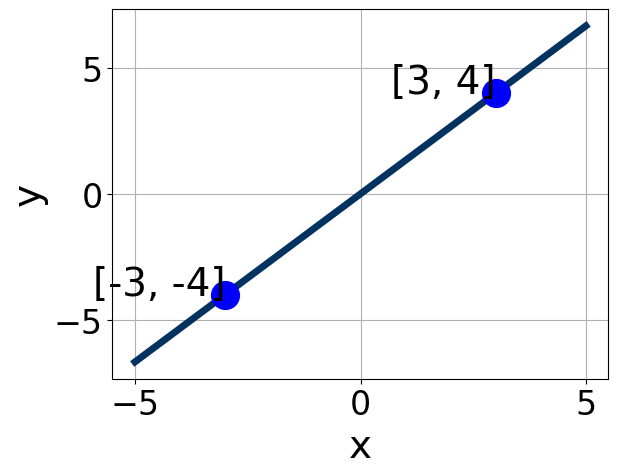
\includegraphics[width=0.5\textwidth]{../Figures/linearGraphToStandardB.png}
\end{center}
\begin{enumerate}[label=\Alph*.]
\item \( A \in [3.21, 5.04], \hspace{3mm} B \in [-5.2, -4.6], \text{ and } \hspace{3mm} C \in [14, 22] \)
\item \( A \in [3.21, 5.04], \hspace{3mm} B \in [4.1, 5.1], \text{ and } \hspace{3mm} C \in [-17, -10] \)
\item \( A \in [-1.23, -0.29], \hspace{3mm} B \in [0.9, 2.1], \text{ and } \hspace{3mm} C \in [-4, 1] \)
\item \( A \in [-4.1, -3.44], \hspace{3mm} B \in [4.1, 5.1], \text{ and } \hspace{3mm} C \in [-17, -10] \)
\item \( A \in [-1.23, -0.29], \hspace{3mm} B \in [-2.7, 0.2], \text{ and } \hspace{3mm} C \in [-1, 4] \)

\end{enumerate} }
\litem{
Write the equation of the line in the graph below in Standard form $Ax+By=C$. Then, choose the intervals that contain $A, B, \text{ and } C$.
\begin{center}
    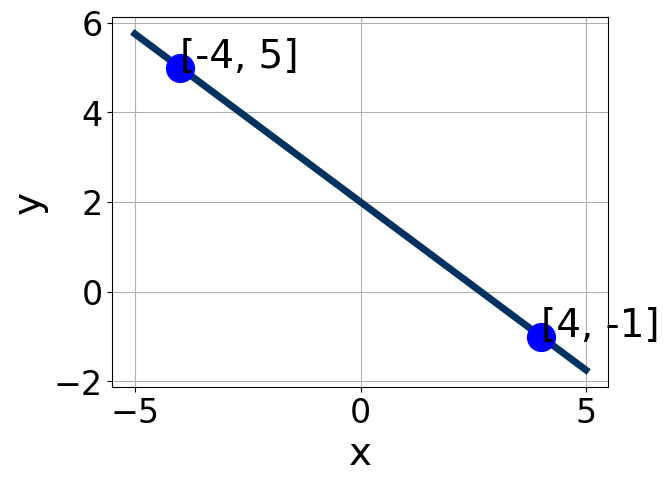
\includegraphics[width=0.5\textwidth]{../Figures/linearGraphToStandardCopyB.png}
\end{center}
\begin{enumerate}[label=\Alph*.]
\item \( A \in [-5, -0.7], \hspace{3mm} B \in [-4.2, -3.2], \text{ and } \hspace{3mm} C \in [-8.2, -5.9] \)
\item \( A \in [2.6, 3.5], \hspace{3mm} B \in [-4.2, -3.2], \text{ and } \hspace{3mm} C \in [-8.2, -5.9] \)
\item \( A \in [-2.4, 2.1], \hspace{3mm} B \in [0.76, 3.5], \text{ and } \hspace{3mm} C \in [0.2, 2.1] \)
\item \( A \in [-2.4, 2.1], \hspace{3mm} B \in [-1.18, -0.31], \text{ and } \hspace{3mm} C \in [-3.8, -0.2] \)
\item \( A \in [2.6, 3.5], \hspace{3mm} B \in [3.15, 4.91], \text{ and } \hspace{3mm} C \in [7.5, 8.9] \)

\end{enumerate} }
\litem{
Solve the equation below. Then, choose the interval that contains the solution.\[ -5(-4x -2) = -11(-12x + 14) \]\begin{enumerate}[label=\Alph*.]
\item \( x \in [1.21, 1.3] \)
\item \( x \in [-1.4, -1.25] \)
\item \( x \in [0.93, 1.04] \)
\item \( x \in [1.46, 1.55] \)
\item \( \text{There are no real solutions.} \)

\end{enumerate} }
\litem{
First, find the equation of the line containing the two points below. Then, write the equation as $ y=mx+b $ and choose the intervals that contain $m$ and $b$.\[ (-11, 4) \text{ and } (2, -3) \]\begin{enumerate}[label=\Alph*.]
\item \( m \in [-2, 0.5] \hspace*{3mm} b \in [1.42, 2.11] \)
\item \( m \in [-2, 0.5] \hspace*{3mm} b \in [14.36, 15.3] \)
\item \( m \in [-2, 0.5] \hspace*{3mm} b \in [-2.67, -1.25] \)
\item \( m \in [0.4, 2.6] \hspace*{3mm} b \in [-4.08, -3.84] \)
\item \( m \in [-2, 0.5] \hspace*{3mm} b \in [-5.41, -4.34] \)

\end{enumerate} }
\litem{
Solve the equation below. Then, choose the interval that contains the solution.\[ -14(17x -18) = -16(9x + 19) \]\begin{enumerate}[label=\Alph*.]
\item \( x \in [-0.3, -0.07] \)
\item \( x \in [5.62, 6.41] \)
\item \( x \in [-1.17, -0.47] \)
\item \( x \in [0.42, 0.98] \)
\item \( \text{There are no real solutions.} \)

\end{enumerate} }
\litem{
First, find the equation of the line containing the two points below. Then, write the equation as $ y=mx+b $ and choose the intervals that contain $m$ and $b$.\[ (10, -10) \text{ and } (-8, -8) \]\begin{enumerate}[label=\Alph*.]
\item \( m \in [-0.24, 0.03] \hspace*{3mm} b \in [-2.5, 2.3] \)
\item \( m \in [-0.24, 0.03] \hspace*{3mm} b \in [-9.3, -7.4] \)
\item \( m \in [0.04, 0.4] \hspace*{3mm} b \in [-7.4, -7] \)
\item \( m \in [-0.24, 0.03] \hspace*{3mm} b \in [6.1, 9.6] \)
\item \( m \in [-0.24, 0.03] \hspace*{3mm} b \in [-20.2, -19.7] \)

\end{enumerate} }
\litem{
Find the equation of the line described below. Write the linear equation as $ y=mx+b $ and choose the intervals that contain $m$ and $b$.\[ \text{Parallel to } 3 x - 8 y = 5 \text{ and passing through the point } (5, 6). \]\begin{enumerate}[label=\Alph*.]
\item \( m \in [-0.05, 0.52] \hspace*{3mm} b \in [4.12, 5.12] \)
\item \( m \in [-0.4, 0.35] \hspace*{3mm} b \in [5.88, 10.88] \)
\item \( m \in [-0.05, 0.52] \hspace*{3mm} b \in [-5.12, -3.12] \)
\item \( m \in [1.94, 2.71] \hspace*{3mm} b \in [4.12, 5.12] \)
\item \( m \in [-0.05, 0.52] \hspace*{3mm} b \in [-2, 3] \)

\end{enumerate} }
\litem{
Solve the linear equation below. Then, choose the interval that contains the solution.\[ \frac{-3x + 9}{2} - \frac{-4x -6}{5} = \frac{-5x + 4}{4} \]\begin{enumerate}[label=\Alph*.]
\item \( x \in [-9.1, -7.6] \)
\item \( x \in [-2.6, 1.1] \)
\item \( x \in [-5.7, -3] \)
\item \( x \in [-20.6, -17.8] \)
\item \( \text{There are no real solutions.} \)

\end{enumerate} }
\litem{
Find the equation of the line described below. Write the linear equation as $ y=mx+b $ and choose the intervals that contain $m$ and $b$.\[ \text{Parallel to } 4 x - 7 y = 12 \text{ and passing through the point } (-10, 5). \]\begin{enumerate}[label=\Alph*.]
\item \( m \in [-1.01, -0.46] \hspace*{3mm} b \in [-2.71, 1.29] \)
\item \( m \in [0.5, 1.21] \hspace*{3mm} b \in [14, 17] \)
\item \( m \in [0.5, 1.21] \hspace*{3mm} b \in [-11.71, -9.71] \)
\item \( m \in [0.5, 1.21] \hspace*{3mm} b \in [10.71, 13.71] \)
\item \( m \in [1.58, 2.47] \hspace*{3mm} b \in [10.71, 13.71] \)

\end{enumerate} }
\end{enumerate}

\end{document}